\documentclass[dvipdfmx]{jarticle}
\hoffset=-25mm
\voffset=-20mm
\pagestyle{empty}
\usepackage{graphicx}
\usepackage{color}
\usepackage{latexsym}
\usepackage{amssymb}
\usepackage{wrapfig}
\usepackage{xcolor}
\usepackage{tikz}
\usetikzlibrary{calc,shapes}
\usepackage{fancyvrb}
\usepackage{url}
\newcounter{coffee}
\newcounter{bean}
\newcounter{figcnt}
\newcommand{\tuple}[1]{\langle{#1}\rangle}

\setlength{\textheight}{25.5cm}
\setlength{\textwidth}{17cm}

%\deflinenumfalse % 定義番号を表示しない

\usepackage{amsmath}	% required for `\cases' (yatex added)
\begin{document}
\begin{flushright}
    \verb|2026/11/24|
\end{flushright}
\begin{center}
    {\Large\bf コンパイラ 第８回演習課題}
\end{center}
\begin{itemize}
    \item TACTの課題の添付ファイルとしてPDFファイルで提出すること．
    \item 手書きレポートをPDFとして提出する方法は講義webサイトを
          参照\footnote{\url{https://sites.google.com/sqlab.jp/26compiler/how-to-make-report}}すること．
    \item 提出期限: {12月3日（木）23:55}（金曜でないので注意）
\end{itemize}

\begin{list}{[\arabic{coffee}]}{\usecounter{coffee}}
    \item 前回(11月13日出題)課題の[2](4)の$\varphi$関数を消去したフローグラフを示せ．
    \item 次の基本ブロックに対して，入口では\verb|a|,\verb|b|が生きていて，出口では\verb|d|,\verb|e|が生きているとする．
    \begin{center}
    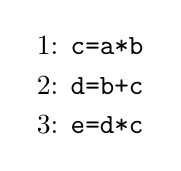
\begin{tikzpicture}
    \node[anchor=west] at (0,0) {1: \verb|c=a*b|};
    \node[anchor=west] at (0,-0.5) {2: \verb|d=b+c|};
    \node[anchor=west] at (0,-1) {3: \verb|e=d*c|};
    \end{tikzpicture}
    \end{center}
    \begin{list}{(\arabic{bean})}{\usecounter{bean}}
        \item 各行の前後において，生存している変数の集合を示せ．
        \item \verb|a|,...,\verb|e| をノードとする干渉グラフを示せ．
        \item 干渉グラフを彩色せよ．
        \item \verb|ADD| $R_1$,$R_2$ および \verb|MUL| $R_1$,$R_2$を用いてレジスタ割当をした機械語を示せ．$R_1$と$R_2$に加算，乗算を行って結果を$R_1$に格納するものとする．
    \end{list}
\end{list}
\end{document}